\chapter{Moyens de défense}
Grâce à l'outil réalisé, nous sommes en mesure de tester l'efficacité de différents moyens de défense.
Le but de ce chapitre est donc de déterminer quelle est la meilleure protection disponible dans Firefox contre les différents types de trackers détectables par l'outil.

\section{Extensions des navigateurs}
\label{extensions_navigateurs}
Certaines extensions de navigateurs ont été développées afin de préserver la vie privée des utilisateurs.
Dans cette section, plusieurs de ces extensions disponibles pour Firefox vont être testées selon une expérience ponctuelle (voir \autoref{experience_ponctuelle}).
\newline

Le \textit{crawler} a chaque fois été configuré pour analyser sur le TOP 1000 du classement Alexa \cite{AlexaTop} du 16 mai 2014. La méthodologie pour la préparation de chaque analyse est la suivante:
\begin{itemize}
  \item chaque profil Firefox est créé expressément pour chaque analyse
  \item les extensions Firebug et NetExport sont installées
  \item l'extension NetExport est modifiée (voir \autoref{changements_extensions})
  \item l'extension devant être testée est installée et configurée
  \newline
\end{itemize}

Le \textit{crawler} génère ainsi les fichiers HTTP Archive et détermine le nombre de cookies Flash créés par chaque site.
\newline

Pour terminer, le \textit{parser} traite les fichiers HTTP Archive afin de fournir les données essentielles à l'élaboration des résultats. Le \textit{parser} a utilisé la version 303 de la base de données de trackers Ghostery.
\newline

Le but de chaque expérience est de déterminer si le nombre de trackers détectés par le \textit{parser} est effectivement en baisse grâce aux extensions installées. L'ensemble de ces différentes expériences permettra ensuite de déterminer quelle protection semble la meilleure.
\newline

Pour chaque expérience, seul les analyses utilisant la base de données Ghostery ont été réalisées. Suite à la discussion portant sur les deux types d'analyses (\autoref{discussion_analyses}), il semble que les analyses utilisant les données issues de Ghostery soient les plus pertinentes pour les tests d'extensions de Firefox.
\newline

Les résultats sont toujours présentés dans un même modèle de tableau :\\

\begin{tabular}{ c | p{6cm} | c | c || c | }
   Rang & Répartition des trackers & \# & \% & Evolution \\
   \hline
   \hline
   1 & Ghostery et critères triés &  &  & Pourcentage \\
   \vdots & en ordre décroissant par & \vdots & \vdots & par rapport \\
   6 & rapport au nombre de trackers &  &  & à la référence \\
   \hline
    & TOTAL &  & - & \\
   \hline
\end{tabular}
\\[1cm]
Notez que la somme des pourcentages de répartition des trackers dans le tableau peut ne pas être exactement de 100\% à cause des arrondis.
\newline

Afin de ne pas surcharger ce chapitre de graphiques, les types MIME des éléments détectés par la base de données Ghostery n'ont pas été inclus mais leurs résultats sont énoncés dans les analyses de chaque expérience. Les types \textit{application/x-javascript}, \textit{application/javascript} et \textit{text/javascript} ont été rassemblés sous le nom \textit{JavaScript} car ils représentent le même type de trackers. Ils sont présentés sous cette forme :\\

\begin{tabular}{ c | p{5cm} | c | c | c | }
   Rang & Types MIME (Ghostery) & \# & \% & Evolution\\
   \hline
   \hline
   1 & Types MIME triés &  &  & Pourcentage \\
   \vdots & en ordre décroissant & \vdots & \vdots & par rapport \\
   5 &  &  &  & à la référence \\
   \hline
\end{tabular}
\\[1cm]

Etant donné que seuls les 5 premiers types MIME sont présents dans le tableau, il est normal que la somme des pourcentages n'atteigne pas 100\%.
\newpage

\subsection{Données de référence}
Pour rappel, voici les données de référence du chapitre précédent (Figures \ref{exp_normal_ghostery} et \ref{exp_normal_ghostery_mimetype}), mises sour forme de tableaux :\\

\begin{tabular}{ c | p{5cm} | c | c | }
   Rang & Répartition des trackers & \# & \% \\
   \hline
   \hline
   1 & Ghostery & 24627 & 83,76 \\
   2 & URL avec paramètres & 1350 & 4,59 \\
   3 & Tracking pixels & 1212 & 4,12 \\
   4 & JavaScript avec paramètres & 1079 & 3,67 \\
   5 & Cookies & 888 & 3,02 \\
   6 & Flash & 246 & 0,84 \\
   \hline
    & TOTAL & 29402 \\
   \cline{1-3}
\end{tabular}
\\[1cm]

\begin{tabular}{ c | p{5cm} | c | c | }
   Rang & Types MIME (Ghostery) & \# & \% \\
   \hline
   \hline
   1 & Images .gif & 7456 & 30,28 \\
   2 & JavaScript & 6959 & 28,26 \\
   3 & HTML & 4830 & 19,61 \\
   4 & Type inconnu & 1644 & 6,68 \\
   5 & Texte & 1069 & 4,34 \\
   \hline
\end{tabular}

\subsection{Adblock Plus}
\subsubsection{Présentation}
Adblock Plus \footnote{\url{https://adblockplus.org/}} est une extension disponible pour Firefox, Google Chrome, Opera, Safari, Internet Explorer et Android. Son fonctionnement repose sur des filtres installés au choix par l'utilisateur. Le but d'Adblock Plus est de bloquer les publicités intrusives et n'autoriser que les publicités jugées acceptables. En effet, les sites dont les publicités sont considérées comme acceptables (des critères stricts ont été définis par Adblock Plus) peuvent demander à être intégrés dans une liste d'exceptions afin de rendre leurs publicités visibles par les utilisateurs. Cependant, l'utilisateur est libre d'afficher ces publicités. De plus, il est possible de créer des listes personnalisées.

Adblock propose des listes par défaut régulièrement mises à jour. Certaines concernent les publicités indésirables de façon générale et d'autres sont spécifiques à des langues. Plusieurs miroirs existent et proposent de bloquer des types précis d'éléments (modules de réseaux sociaux par exemple). Un de ces miroirs connus est Fanboy \footnote{\url{https://www.fanboy.co.nz/}}, il propose plusieurs listes dont certaines bloquent des éléments qui tracent les utilisateurs. Les listes ont généralement une durée de vie de 4 jours.

\subsubsection{Configuration de l'extension}
Etant donné que les résultats peuvent varier en fonction des filtres installés, trois expériences ont été réalisées avec cette extension.

La première utilise les paramètres par défaut : le filtre de base (Easylist) et un filtre basé sur la langue.

La seconde expérience est basée sur les mêmes réglages que la première mais bloque également les publicités dites acceptables par Adblock.

La troisième utilise un filtre de blocage plus complet. Il s'agit de la liste "Ultimate" Fanboy \footnote{\url{http://www.fanboy.co.nz/filters.html}}, cette liste inclut les éléments suivants: Easylist, Easyprivacy, Enhanced Trackers List and Annoyances List.

Notez que des profils Firefox différents ont été configurés pour réaliser les différentes expériences afin d'éviter une quelconque influence entre elles.

\subsubsection{Résultats de la première expérience - \autoref{exp-AdblockDefault-ghostery}}
\begin{figure}[!h]
	\centering
	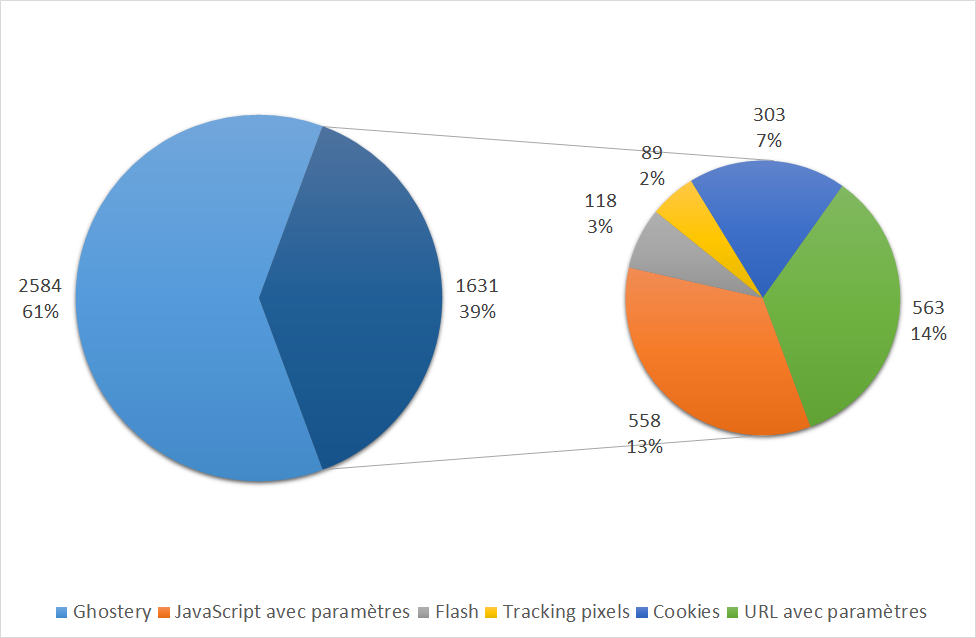
\includegraphics[scale=.6]{resultats/ANALYSES/Images/AdblockDefault-Ghostery.png}
	\caption{\label{exp-AdblockDefault-ghostery}Répartition des trackers par catégorie.}
\end{figure}

L'extension a laissé passer 2584 trackers connus de la base de données Ghostery et 1631 éléments ont été identifiés comme trackers selon les critères de l'outil.\\

\begin{tabular}{ c | p{5cm} | c | c || c | }
   Rang & Répartition des trackers & \# & \% & Evolution \\
   \hline
   \hline
   1 & Ghostery & 2584 & 61,30 & - 89,51\% \\
   2 & URL avec paramètres & 563 & 13,36 & - 58,30\% \\
   3 & JavaScript avec paramètres & 558 & 13,24 & - 48,29\% \\
   4 & Cookies & 303 & 7,19 & - 65,88\% \\
   5 & Flash & 118 & 2,80 & - 52,03\% \\
   6 & Tracking pixels & 89 & 2,11 & - 92,66\% \\
   \hline
    & TOTAL & 4215 & - & - 85,66\%\\
   \hline
\end{tabular}
\\[1cm]

\begin{tabular}{ c | p{5cm} | c | c | c | }
   Rang & Types MIME (Ghostery) & \# & \% & Evolution\\
   \hline
   \hline
   1 & JavaScript & 1136 & 43,96 & - 83,68\% \\
   2 & Images .png & 396 & 15,33 & - 59,09\% \\
   3 & HTML & 322 & 12,46 & - 93,33\% \\
   4 & Images .jpeg & 300 & 11,61 & - 56,08\% \\
   5 & Images .gif & 151 & 5,84 & -97,97\% \\
   \hline
\end{tabular}
\\[.3cm]

Deux baisses flagrantes sont constatées pour les pixels de traçage et les trackers connus de Ghostery. Dans ces derniers, ce sont principalement les images .gif, les requêtes de ressources HTML et les JavaScript qui sont bloqués par Adblock.

%Concernant les trackers bloqués par la base de données Ghostery, 1136 sont du JavaScript (en rassemblant les types \textit{application/x-javascript} (645), \textit{application/javascript} (264) et \textit{text/javascript} (227)). La deuxième position est occupée par les images \textit{.png} (396) et le trio de tête termine avec les images \textit{.jpeg} (300). Les trackers sous la forme d'images {.gif} semblent avoir bien été bloqués car ils ne sont que 151. Notons également la présence de 149 éléments de type {.css} jouant le rôle de trackers.

%Les 1631 autres éléments (graphique en secteurs visible à droite) sont constitués essentiellement d'URL avec une chaîne de requête (563 éléments, 14\%), de 558 codes JavaScript avec paramètres (13\%) et de réponses créant un cookie tiers (303, 7\%). Peu de pixels de traçage ont été détectés car ils ne sont qu'au nombre de 89 (2\%). Par contre, 118 ressources Flash ont été chargées depuis un domaine externe (3\%).

\subsubsection{Résultats de la seconde expérience - \autoref{exp-AdblockNoAcceptableAds-ghostery}}
\begin{figure}[!h]
	\centering
	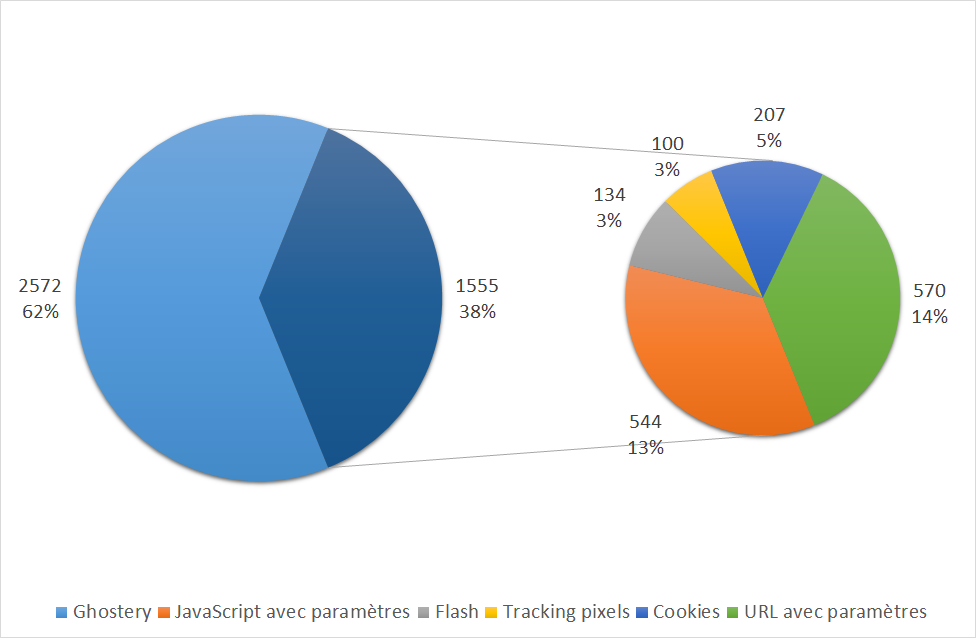
\includegraphics[scale=.6]{resultats/ANALYSES/Images/AdblockNoAcceptableAds-Ghostery.png}
	\caption{\label{exp-AdblockNoAcceptableAds-ghostery}Répartition des trackers par catégorie.}
\end{figure}

L'extension a laissé passer 2572 trackers connus de la base de données Ghostery et 1555 éléments ont été identifiés comme trackers selon les critères de l'outil.\\

\begin{tabular}{ c | p{5cm} | c | c || c | }
   Rang & Répartition des trackers & \# & \% & Evolution \\
   \hline
   \hline
   1 & Ghostery & 2572 & 62,32 & - 89,56\% \\
   2 & URL avec paramètres & 570 & 13,81 & - 57,78\% \\
   3 & JavaScript avec paramètres & 544 & 13,18 & - 49,58\% \\
   4 & Cookies & 207 & 5,02 & - 76,69\% \\
   5 & Flash & 134 & 3,25 & - 45,53\% \\
   6 & Tracking pixels & 100 & 2,42 & - 91,75\% \\
   \hline
    & TOTAL & 4127 & - & - 85,96\%\\
   \hline
\end{tabular}
\\[1cm]

\begin{tabular}{ c | p{5cm} | c | c | c | }
   Rang & Types MIME (Ghostery) & \# & \% & Evolution\\
   \hline
   \hline
   1 & JavaScript & 1134 & 44,09 & - 83,70\% \\
   2 & Images .png & 407 & 15,82 & - 57,95\% \\
   4 & HTML & 330 & 12,83 & - 93,17\% \\
   4 & Images .jpeg & 245 & 9,53 & - 64,13\% \\
   5 & Images .gif & 161 & 6,26 & - 97,84\% \\
   \hline
\end{tabular}
\\[.3cm]

Le fait de bloquer les publicités dites acceptables par les développeurs d'Adblock fait baisser un peu plus le niveau de trackers détectés : on passe de 4215 à 4127 trackers. Cette baisse est essentiellement causée par la diminution du nombre de réponses HTTP créant un cookie tiers (on diminue de 300 à 207). On constate également un nombre légèrement supérieur pour les ressources Flash, les pixels de traçage et les URL avec paramètres. Après vérification du log du \textit{parser}, 4 fichiers HTTP Archive ont été analysés en plus, ce qui provoque probablement ces légères hausses.

\subsubsection{Résultats de la troisième expérience - \autoref{exp-AdblockFanboyUltimate-ghostery}}
\begin{figure}[!h]
	\centering
	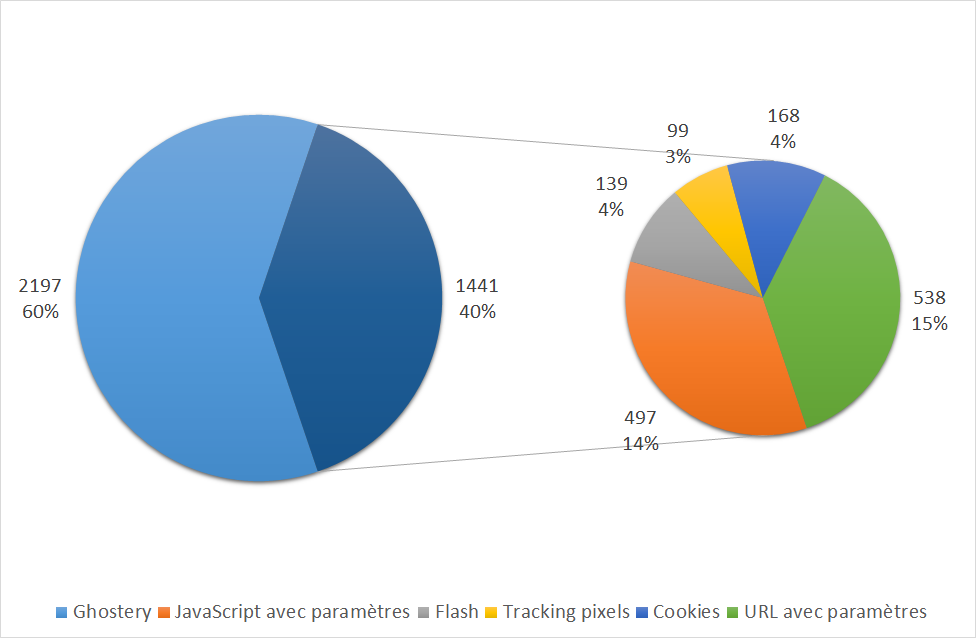
\includegraphics[scale=.6]{resultats/ANALYSES/Images/AdblockFanboyUltimate-Ghostery.png}
	\caption{\label{exp-AdblockFanboyUltimate-ghostery}Répartition des trackers par catégorie.}
\end{figure}

L'extension a laissé passer 2197 trackers connus de la base de données Ghostery et 1441 éléments ont été identifiés comme trackers selon les critères de l'outil.\\

\begin{tabular}{ c | p{5cm} | c | c || c | }
   Rang & Répartition des trackers & \# & \% & Evolution \\
   \hline
   \hline
   1 & Ghostery & 2197 & 60,39 & - 91,08\% \\
   2 & URL avec paramètres & 538 & 14,79 & - 60,15\% \\
   3 & JavaScript avec paramètres & 497 & 13,66 & - 53,94\% \\
   4 & Cookies & 168 & 4,62 & - 81,08\% \\
   5 & Flash & 139 & 3,82 & - 43,50\% \\
   6 & Tracking pixels & 99 & 2,72 & - 91,83\% \\
   \hline
    & TOTAL & 3638 & - & - 87,63\%\\
   \hline
\end{tabular}
\\[1cm]

\begin{tabular}{ c | p{5cm} | c | c | c | }
   Rang & Types MIME (Ghostery) & \# & \% & Evolution\\
   \hline
   \hline
   1 & JavaScript & 764 & 34,77 & - 89,02\% \\
   2 & Images .png & 373 & 16,98 & - 61,47\% \\
   3 & HTML & 318 & 14,47 & - 93,42\% \\
   4 & Images .jpeg & 316 & 14,38 & - 53,73\% \\
   5 & Images .gif & 152 & 6,92 & - 97,96\% \\
   \hline
\end{tabular}
\\[.3cm]

L'utilisation de la liste Fanboy Ultimate fait baisser davantage le nombre de trackers car on passe de 4127 pour l'expérience précédente (4215 pour la configuration par défaut d'Adblock) à 3638 trackers détectés. Pour les trackers de la base de données Ghostery, la baisse vient principalement du JavaScript avec une baisse de 1134 (1136 pour la configuration par défaut d'Adblock) à 764 codes JavaScript connus comme trackers ayant été détectés. Concernant les autres critères, une légère baisse des URL et JavaScript avec des paramètres est visible ainsi que pour les cookies.

%%%%%%%%%%
\subsection{DoNotTrackMe}
\subsubsection{Présentation}
DoNotTrackMe \footnote{\url{https://www.abine.com/donottrackme.html}} est une extension disponible pour Google Chrome, Firefox, Safari, Opera et Internet Explorer.
Elle bloque les trackers de différents types de sociétés (régies publicitaires, réseaux sociaux et sociétés qui récupèrent des données sur la navigation des utilisateurs). Il est expliqué sur le site de l'extension que son but n'est pas de bloquer toutes les publicités mais plutôt de bloquer les publicités ciblées qui utilisent des informations personnelles. Son fonctionnement repose sur une base de données de trackers. A chaque page ouverte dans le navigateur, l'extension vérifie les ressources qui sont chargées et bloque celles qui sont connues comme trackers.

\subsubsection{Configuration de l'extension}
L'extension n'a pas été configurée, les paramètres par défaut ont été laissés d'application. A vrai dire, les options de configuration sont assez rudimentaires. L'extension possède un écran de contrôle qui compte le nombre de trackers bloqués. Un compte premium est également proposé mais il n'est pas intéressant vu les fonctionnalités recherchées au sein de l'expérience.

\subsubsection{Résultats - \autoref{exp-DoNotTrackMe-ghostery}}
\begin{figure}[!h]
	\centering
	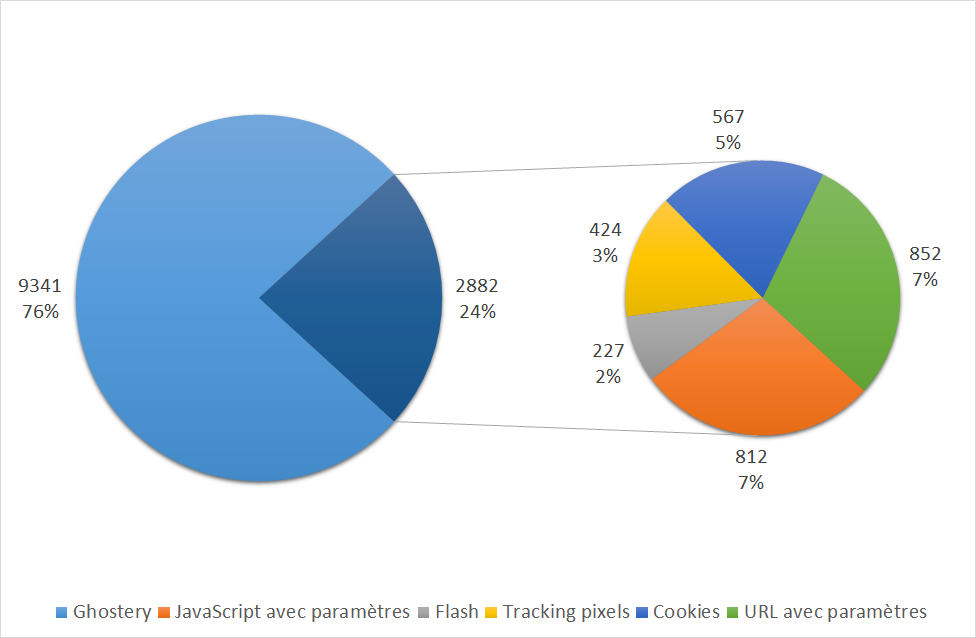
\includegraphics[scale=.6]{resultats/ANALYSES/Images/DoNotTrackMe-Ghostery.png}
	\caption{\label{exp-DoNotTrackMe-ghostery}Répartition des trackers par catégorie.}
\end{figure}

L'extension a laissé passer 9341 trackers connus de la base de données Ghostery et 2882 éléments ont été identifiés comme trackers selon les critères de l'outil.\\

\begin{tabular}{ c | p{5cm} | c | c || c | }
   Rang & Répartition des trackers & \# & \% & Evolution \\
   \hline
   \hline
   1 & Ghostery & 9341 & 76,42 & - 62,07\% \\
   2 & URL avec paramètres & 852 & 6,97 & - 36,89\% \\
   3 & JavaScript avec paramètres & 812 & 6,64 & - 24,75\% \\
   4 & Cookies & 567 & 4,64 & - 36,15\% \\
   5 & Tracking pixels & 424 & 3,47 & - 65,02\% \\
   6 & Flash & 227 & 1,86 & - 7,72\% \\
   \hline
    & TOTAL & 12223 & - & - 58,43\%\\
   \hline
\end{tabular}
\\[1cm]

\begin{tabular}{ c | p{5cm} | c | c | c | }
   Rang & Types MIME (Ghostery) & \# & \% & Evolution\\
   \hline
   \hline
   1 & JavaScript & 3441 & 36,84 & - 50,55\% \\
   2 & Images .gif & 2124 & 22,74 & - 71,51\% \\
   3 & HTML & 1400 & 14,99 & - 71,01\% \\
   4 & Type inconnu & 529 & 5,66 & - 67,82\% \\
   5 & Images .png & 517 & 5,53 & - 46,59\% \\
   \hline
\end{tabular}
\\[.3cm]

L'extension offre une protection relativement moyenne car elle ne bloque que 58,43\% des trackers par rapport à l'expérience de référence. Elle bloque cependant 65,02\% de pixels de traçage et 62,07\% des trackers connus par Ghostery. Dans ces derniers, ce sont les pixels de traçage (71,51\%) et les URL avec une chaîne de requête qui sont proportionnellement les plus bloqués (71,01\% pour le type HTML et 67,82\% pour les types inconnus). Quant aux codes JavaScript, ils sont en tête avec 3441 trackers bloqués.

%%%%%%%%%%
\subsection{Ghostery}
\subsubsection{Présentation}
Ghostery \footnote{\url{https://www.ghostery.com}} est une extension disponible pour Firefox, Google Chrome, Opera et Safari. Son fonctionnement repose sur une base de données de trackers alimentée par les retours des utilisateurs de l'extension. Cette base de données est régulièrement mise à jour. Evidon, la société qui possède Ghostery, a fait momentanément parler d'elle car elle a des contrats avec certaines entreprises. Certains lui reprochaient alors de vendre les informations reçues des utilisateurs via son programme Ghostrank. Sur leur site, les développeurs de Ghostery assurent ne pas vendre d'informations personnelles. Il faut noter qu'il est possible d'utiliser Ghostery sans activer Ghostrank.

\subsubsection{Configuration de l'extension}
L'extension a été activée avec tous les trackers et tous les cookies sélectionnés.

\subsubsection{Résultats - \autoref{exp-Ghostery-ghostery}}
\begin{figure}[!h]
	\centering
	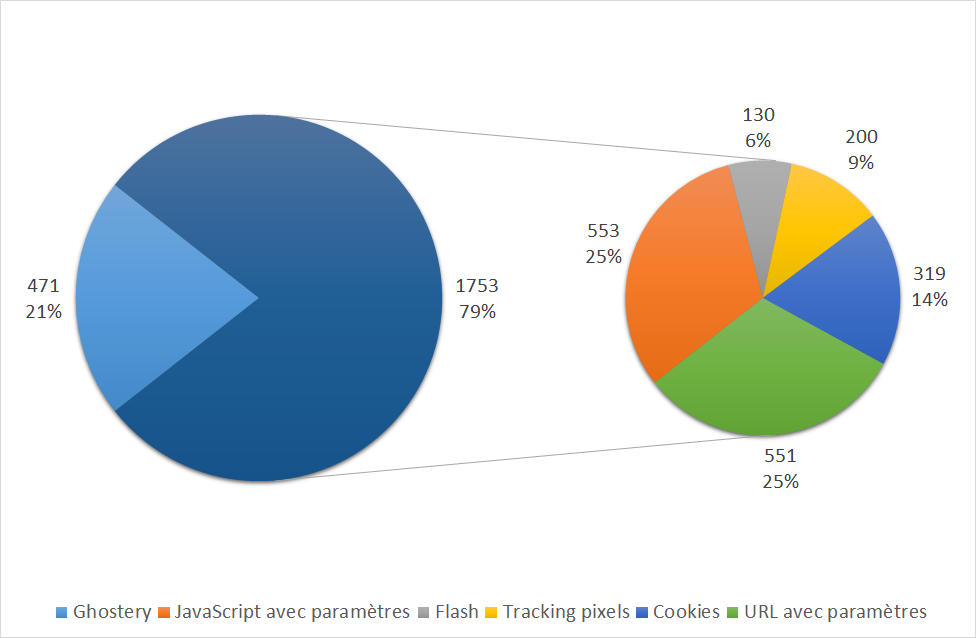
\includegraphics[scale=.6]{resultats/ANALYSES/Images/Ghostery-Ghostery.png}
	\caption{\label{exp-Ghostery-ghostery}Répartition des trackers par catégorie.}
\end{figure}

L'extension a laissé passer 471 trackers connus de la base de données Ghostery et 1753 éléments ont été identifiés comme trackers selon les critères de l'outil.\\

\begin{tabular}{ c | p{5cm} | c | c || c | }
   Rang & Répartition des trackers & \# & \% & Evolution \\
   \hline
   \hline
   1 & JavaScript avec paramètres & 553 & 14,53 & - 48,75\% \\
   2 & URL avec paramètres & 551 & 14,48 & - 59,19\% \\
   3 & Ghostery & 471 & 12,38 & - 98,09\% \\
   4 & Cookies & 319 & 8,38 & - 64,08\% \\
   5 & Tracking pixels & 200 & 5,25 & - 83,50\% \\
   6 & Flash & 130 & 3,42 & - 47,15\% \\
   \hline
    & TOTAL & 2224 & - & - 92,44\%\\
   \hline
\end{tabular}
\\[1cm]

\begin{tabular}{ c | p{5cm} | c | c | c | }
   Rang & Types MIME (Ghostery) & \# & \% & Evolution\\
   \hline
   \hline
   1 & Images .png & 111 & 23,57 & - 88,53\% \\
   2 & Images .jpeg & 92 & 19,53 & - 86,53\% \\
   3 & JavaScript & 86 & 18,26 & - 98,76\% \\
   4 & Images .gif & 62 & 13,16 & - 99,17\% \\
   5 & HTML & 56 & 11,89 & - 98,84\% \\
   \hline
\end{tabular}
\\[.3cm]

Les résultats de l'analyse ont été assez étonnants car ils montrent qu'une partie des trackers n'est pas bloquée par Ghostery alors qu'ils sont bien présents dans la base de données. Ils sont détectés par le \textit{parser} qui utilise la même base de données. Une analyse plus poussée sur les liens non bloqués a été effectuée. Le constat était que Ghostery ne bloque pas les trackers du site visité (les trackers "first-party"). Après une recherche, la justification a été trouvé sur un billet de blog \footnote{\url{https://purplebox.ghostery.com/post/1016021484}} des développeurs de l'extension. La raison principale est que bloquer ces trackers peut entraîner des interférences lors de l'utilisation des fonctionnalités du site.

Néanmoins, l'extension offre une bonne protection car elle bloque 92,44\% des trackers. Les principaux trackers non bloqués sur les sites visités sont les images .png et .jpeg (respectivement 23,57\% et 19,53\%), suivies des JavaScript (18,26\%) et des images .gif (13,16\%).
Concernant les autres critères, les pixels de traçage sont relativement bien bloqués avec un taux de 83,50\%, cela signifie que 200 pixels passent quand même à côté de la base de données Ghostery.

%%%%%%%%%%
\subsection{HTTPS Everywhere}
\subsubsection{Présentation}
HTTPS Everywhere \footnote{\url{https://www.eff.org/https-everywhere}} est une extension disponible pour Firefox, Google Chrome, Opera et Android. Firefox dispose d'une version stable tandis que les autres n'ont accès qu'à une version beta. Le but de cette extension est d'utiliser les connexions HTTPS dès que cela est possible. L'extension repose sur une liste afin de savoir quand passer d'une connexion HTTP vers une connection HTTPS. Par défaut, l'extension contient une liste de règles prédéfinies pour chaque site mais il est également possible de créer ses propres règles.
Grâce à l'utilisation de connections sécurisées, l'extension protège l'utilisateur de certaines attaques. Dès qu'une connection sécurisée peut être établie vers un site, HTTPS Everywhere le fait. Il peut cependant arriver que certaines requêtes vers un site soient en HTTP alors que d'autres sont en HTTPS. L'extension n'est pas en mesure de protéger l'utilisateur si le site ne propose pas de connection HTTPS pour toutes ses ressources.

\subsubsection{Configuration de l'extension}
L'extension a été installée avec ses paramètres par défaut. SSL Observatory n'a pas été activé et aucune règle supplémentaire n'a été ajoutée.

\subsubsection{Résultats - \autoref{exp-HTTPSEverywhere-ghostery}}
\begin{figure}[!h]
	\centering
	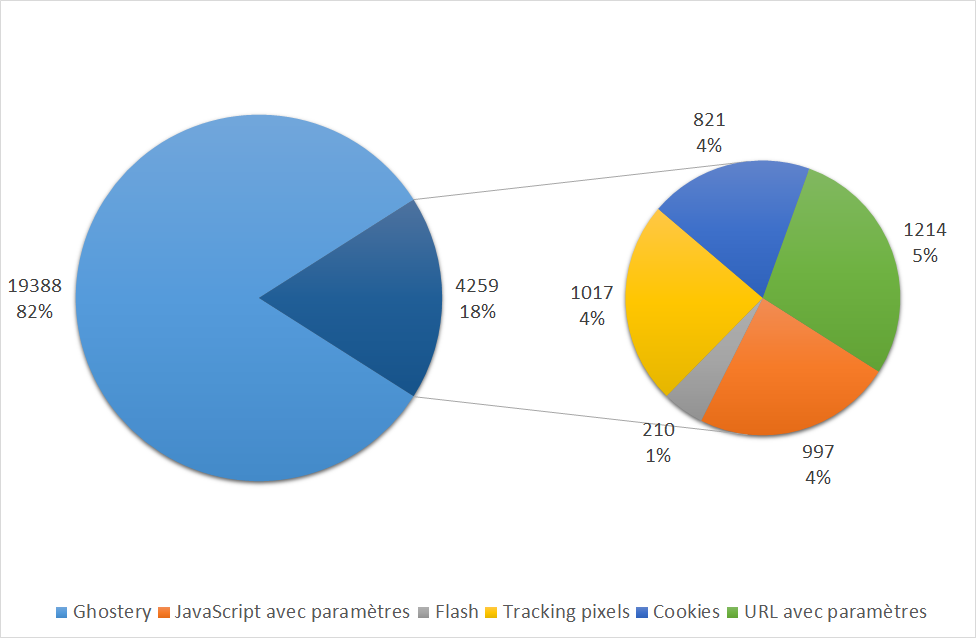
\includegraphics[scale=.6]{resultats/ANALYSES/Images/HTTPSEverywhere-Ghostery.png}
	\caption{\label{exp-HTTPSEverywhere-ghostery}Répartition des trackers par catégorie.}
\end{figure}

L'extension a laissé passer 19388 trackers connus de la base de données Ghostery et 4259 éléments ont été identifiés comme trackers selon les critères de l'outil.\\

\begin{tabular}{ c | p{5cm} | c | c || c | }
   Rang & Répartition des trackers & \# & \% & Evolution \\
   \hline
   \hline
   1 & Ghostery & 19388 & 81,99 & - 21,27\% \\
   2 & URL avec paramètres & 1214 & 5,13 & - 10,07\% \\
   3 & Tracking pixels & 1017 & 4,30 & - 16,09\% \\
   4 & JavaScript avec paramètres & 997 & 4,22 & - 7,60\% \\
   5 & Cookies & 821 & 3,47 & - 7,55\% \\
   6 & Flash & 210 & 0,89 & - 14,63\% \\
   \hline
    & TOTAL & 23647 & - & - 19,57\%\\
   \hline
\end{tabular}
\\[1cm]

\begin{tabular}{ c | p{5cm} | c | c | c | }
   Rang & Types MIME (Ghostery) & \# & \% & Evolution\\
   \hline
   \hline
   1 & Images .gif & 5817 & 30,00 & - 21,98\% \\
   2 & JavaScript & 5659 & 29,19 & - 18,68\% \\
   3 & HTML & 3782 & 19,51 & - 21,70\% \\
   4 & Type inconnu & 1142 & 5,89 & - 30,54\% \\
   5 & Texte & 826 & 4,26 & - 22,73\% \\
   \hline
\end{tabular}
\\[.3cm]

HTTPS Everywhere n'est pas une extension dont le but est de protéger la vie privée mais la motivation pour cette expérience était de voir si le fait de se connecter en HTTPS à des sites avait une incidence sur le nombre de trackers. D'après les résultats, il semble que oui car on observe une baisse de 19,57\% du nombre de trackers par rapport à la référence.


%%%%%%%%%%
\subsection{Priv3}
\subsubsection{Présentation}
Priv3 \footnote{\url{http://priv3.icsi.berkeley.edu/}} est une extension uniquement disponible pour Firefox. Son but est de bloquer le tracking effectué par les réseaux sociaux. Priv3 ne bloque pas complètement toutes les interactions tierces, elle supprime de manière sélective l'inclusion de cookies tiers quand le navigateur récupère du contenu provenant des réseaux sociaux mais les réactive lorsqu'on veut interagir avec les modules des réseaux sociaux.
\newline

L'extension gère les réseaux sociaux suivants: Facebook, Twitter, Google+ et LinkedIn. Cependant, elle ne semble plus mise à jour depuis juillet 2011.

\subsubsection{Configuration de l'extension}
Aucun paramètre de configuration n'est disponible pour cette extension.

\subsubsection{Résultats - \autoref{exp-Priv3-ghostery}}
\begin{figure}[!h]
	\centering
	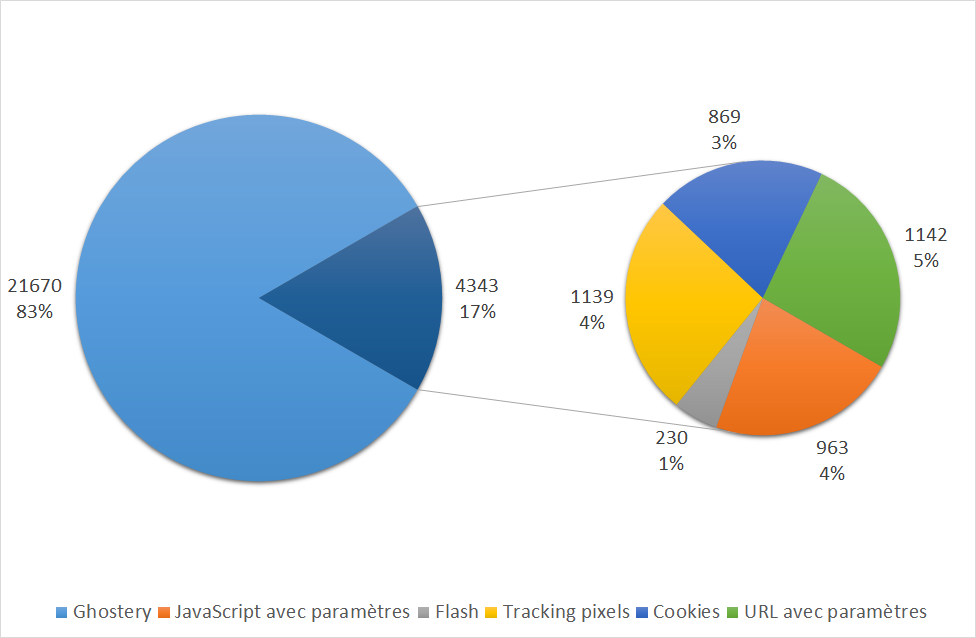
\includegraphics[scale=.6]{resultats/ANALYSES/Images/Priv3-Ghostery.png}
	\caption{\label{exp-Priv3-ghostery}Répartition des trackers par catégorie.}
\end{figure}

L'extension a laissé passer 21670 trackers connus de la base de données Ghostery et 4343 éléments ont été identifiés comme trackers selon les critères de l'outil.\\

\begin{tabular}{ c | p{5cm} | c | c || c | }
   Rang & Répartition des trackers & \# & \% & Evolution \\
   \hline
   \hline
   1 & Ghostery & 21670 & 83,30 & - 12,01\% \\
   2 & URL avec paramètres & 1142 & 4,39 & - 15,41\% \\
   3 & Tracking pixels & 1139 & 4,38 & - 6,02\% \\
   4 & JavaScript avec paramètres & 963 & 3,70 & - 10,75\% \\
   5 & Cookies & 869 & 3,34 & - 2,14\% \\
   6 & Flash & 230 & 0,88 & - 6,50\% \\
   \hline
    & TOTAL & 26013 & - & - 11,53\%\\
   \hline
\end{tabular}
\\[1cm]

\begin{tabular}{ c | p{5cm} | c | c | c | }
   Rang & Types MIME (Ghostery) & \# & \% & Evolution\\
   \hline
   \hline
   1 & JavaScript & 6484 & 29,92 & - 6,83\% \\
   2 & Images .gif & 6137 & 28,32 & - 17,69\% \\
   3 & HTML & 4307 & 19,88 & - 10,83\% \\
   4 & Type inconnu & 1418 & 6,54 & - 13,75\% \\
   5 & Texte & 954 & 4,40 & - 10,76\% \\
   \hline
\end{tabular}
\\[.3cm]

Priv3 a pour objectif de bloquer les trackers de 4 plateformes de réseaux sociaux. Le but de cette expérience n'était donc pas de voir si l'extension bloquait un nombre important de trackers mais plutôt d'estimer la proportion que représentent les réseaux sociaux dans les trackers. L'extension a bloqué 11,53\% de trackers dont 12,01\% de trackers connus dans la base de données Ghostery. Parmi ces derniers, les images .gif sont proportionnellement les plus bloquées avec une baisse de 17,69\% mais ce sont les JavaScript qui sont en tête avec 6484 trackers de ce type ayant été détectés.


%%%%%%%%%%
\subsection{Privacy Badger}
\subsubsection{Présentation}
Privacy Badger \footnote{\url{https://www.eff.org/privacybadger}} est une extension disponible pour Firefox et Google Chrome, elle est actuellement en version alpha. Son but est de bloquer les trackers de domaines tiers grâce à l'analyse de leur comportement. 
Lors de l'envoi d'une requête, un entête Do Not Track est ajouté et l'extension évalue la probabilité d'être tracké grâce à des heuristiques. L'extension enregistre diverses informations afin d'affiner son fonctionnement en fonction des sites visités. Il faut donc un certain temps pour que l'utilisateur soit mieux protégé.

L'extension contient aussi une liste blanche pour certains domaines qui fournissent des ressources tierces essentielles. A long terme, les développeurs espèrent se séparer de cette liste grâce aux promesses des domaines tiers de respecter Do Not Track. Le but de Privacy Badger n'est pas de bloquer les publicités mais de prévenir les invasions indésirables dans la vie privée des utilisateurs. 
Actuellement, seul le tracking provenant de tiers est bloqué. Dans le futur, les développeurs comptent également ajouter des protections pour les sites visités et ils vont ajouter des contre-mesures pour bloquer les fingerprinters dans une prochaine version.

\subsubsection{Configuration de l'extension}
L'extension est restée configurée avec les paramètres par défaut.

\subsubsection{Résultats - \autoref{exp-PrivacyBadger-ghostery}}
\begin{figure}[!h]
	\centering
	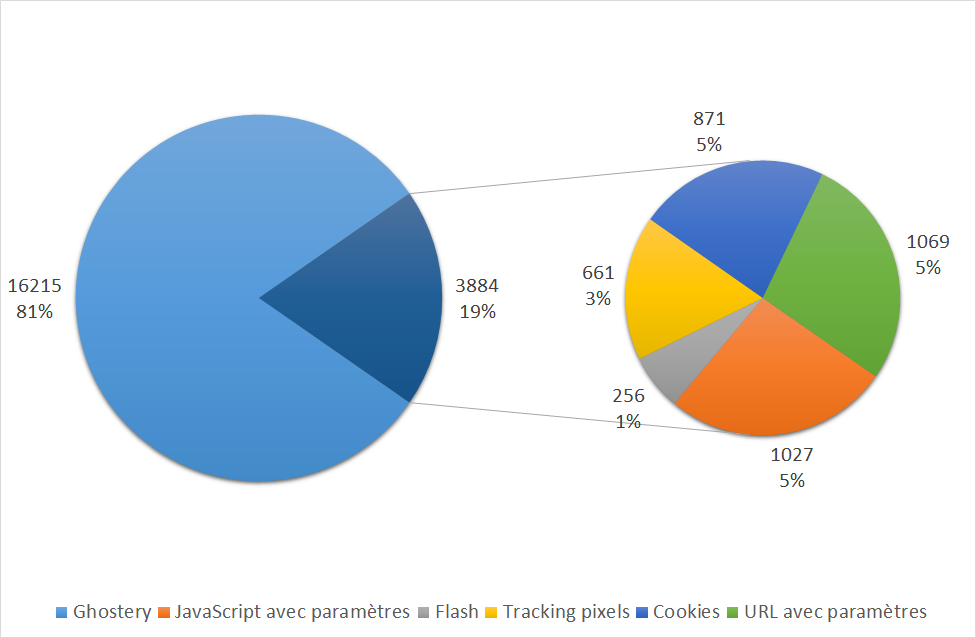
\includegraphics[scale=.6]{resultats/ANALYSES/Images/PrivacyBadger-Ghostery.png}
	\caption{\label{exp-PrivacyBadger-ghostery}Répartition des trackers par catégorie.}
\end{figure}

L'extension a laissé passer 16215 trackers connus de la base de données Ghostery et 3884 éléments ont été identifiés comme trackers selon les critères de l'outil.\\

\begin{tabular}{ c | p{5cm} | c | c || c | }
   Rang & Répartition des trackers & \# & \% & Evolution \\
   \hline
   \hline
   1 & Ghostery & 16215 & 80,68 & - 34,16\% \\
   2 & URL avec paramètres & 1069 & 5,32 & - 20,81\% \\
   3 & JavaScript avec paramètres & 1027 & 5,11 & - 4,82\% \\
   4 & Cookies & 871 & 4,33 & - 1,91\% \\
   5 & Tracking pixels & 661 & 3,29 & - 45,46\% \\
   6 & Flash & 256 & 1,27 & + 4,07\% \\
   \hline
    & TOTAL & 20099 & - & - 31,64\%\\
   \hline
\end{tabular}
\\[1cm]

\begin{tabular}{ c | p{5cm} | c | c | c | }
   Rang & Types MIME (Ghostery) & \# & \% & Evolution\\
   \hline
   \hline
   1 & JavaScript & 5490 & 33,86 & - 21,11\% \\
   2 & Images .gif & 4716 & 29,08 & - 36,75\% \\
   3 & HTML & 2851 & 17,58 & - 40,97\% \\
   4 & Type inconnu & 900 & 5,55 & - 45,26\% \\
   5 & Texte & 601 & 3,71 & - 43,78\% \\
   \hline
\end{tabular}
\\[.3cm]

L'extension bloque un peu moins d'un tiers des trackers. Les trackers connus de Ghostery sont en tête des trackers bloqués avec un nombre de 16215 mais ils ne représentent qu'une baisse de 34,16\% alors que les pixels de traçage sont mieux bloqués avec une baisse de 45,46\%. Le taux de détection de fichiers Flash est en hausse, cela s'explique par un nombre plus important de fichiers analysés (9 fichiers supplémentaires) par le \textit{parser}.


%%%%%%%%%%
\subsection{Adblock \& Ghostery}
\subsubsection{Configuration des extensions}

\subsubsection{Résultats - \autoref{exp-AdblockGhostery-ghostery}}
\begin{figure}[!h]
	\centering
	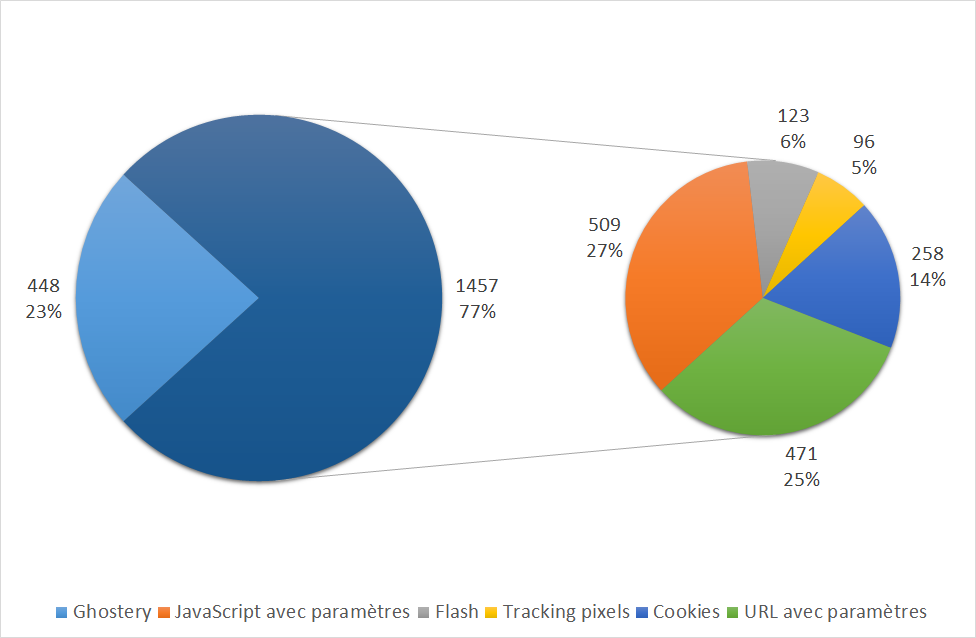
\includegraphics[scale=.6]{resultats/ANALYSES/Images/AdblockGhostery-Ghostery.png}
	\caption{\label{exp-AdblockGhostery-ghostery}Répartition des trackers par catégorie.}
\end{figure}

Les extensions ont laissé passer 448 trackers connus de la base de données Ghostery et 1457 éléments ont été identifiés comme trackers selon les critères de l'outil.\\

\begin{tabular}{ c | p{5cm} | c | c || c | }
   Rang & Répartition des trackers & \# & \% & Evolution \\
   \hline
   \hline
   1 & JavaScript avec paramètres & 509 & 26,72 & - 52,83\% \\
   2 & URL avec paramètres & 471 & 24,72 & - 65,11\% \\
   3 & Ghostery & 448 & 23,52 & - 98,18\% \\
   4 & Cookies & 258 & 13,54 & - 70,95\% \\
   5 & Flash & 123 & 6,46 & - 50,00\% \\
   6 & Tracking pixels & 96 & 5,04 & - 92,08\% \\
   \hline
    & TOTAL & 1905 & - & - 93,52\%\\
   \hline
\end{tabular}
\\[1cm]

\begin{tabular}{ c | p{5cm} | c | c | c | }
   Rang & Types MIME (Ghostery) & \# & \% & Evolution\\
   \hline
   \hline
   1 & Images .jpeg & 176 & 39,29 & - 74,23\% \\
   2 & Images .png & 100 & 22,32 & - 89,67\% \\
   3 & JavaScript & 63 & 14,06 & - 99,09\% \\
   4 & HTML & 39 & 8,71 & - 99,19\% \\
   5 & Images .gif & 31 & 6,92 & - 99,58\% \\
   \hline
\end{tabular}
\\[.3cm]

Cette expérience avait pour but de tester ensemble les deux extensions ayant les meilleurs résultats. Il en ressort que les extensions combinées apportent des résultats encore meilleurs car on atteint un taux de blocage de 93,52\%. Ceci s'explique par le fait qu'Adblock bloque plus de trackers non bloqués par Ghostery, notamment les pixels de traçage et les réponses HTTP qui créent un cookie tiers. D'un autre côté, Ghostery bloque des trackers qui ne sont pas présents dans les listes d'Adblock. Ces deux effets font que le nombre global de trackers diminue davantage afin d'atteindre le meilleur taux de protection.


\section{Do Not Track}
\subsection{Présentation}
Do Not Track \footnote{\url{http://donottrack.us/}} est un entête HTTP qui signale au serveur le souhait de l'utilisateur de ne pas être tracé. Les sites ont le choix d'accepter ce souhait ou de l'ignorer car il n'y a aucun effet contraignant s'ils ne le respectent pas.

L'activation se fait aisément dans les paramètres du navigateur, il ne s'agit que d'une simple case à cocher.

Le but de cette expérience était de voir si les sites respectent cet entête en regardant si le nombre de trackers détectés diminue de façon significative.

\subsection{Résultats - \autoref{exp-DNT-ghostery}}
\begin{figure}[!h]
	\centering
	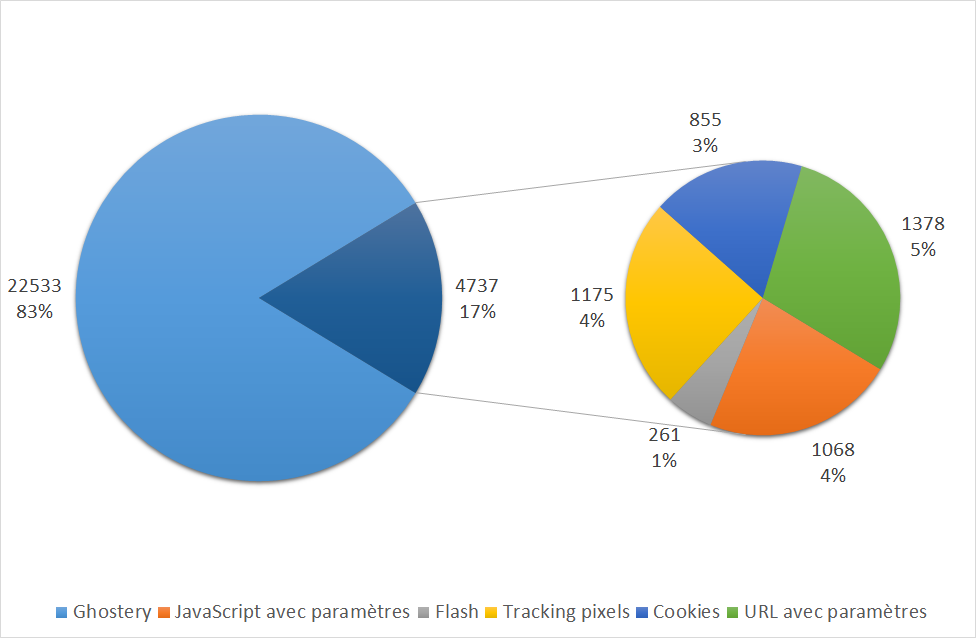
\includegraphics[scale=.6]{resultats/ANALYSES/Images/DNT-Ghostery.png}
	\caption{\label{exp-DNT-ghostery}Répartition des trackers par catégorie.}
\end{figure}

Do Not Track a laissé passer 22533 trackers connus de la base de données Ghostery et 4737 éléments ont été identifiés comme trackers selon les critères de l'outil.\\

\begin{tabular}{ c | p{5cm} | c | c || c | }
   Rang & Répartition des trackers & \# & \% & Evolution \\
   \hline
   \hline
   1 & Ghostery & 22533 & 82,63 & - 8,50\% \\
   2 & URL avec paramètres & 1378 & 5,05 & + 2,07\% \\
   3 & Tracking pixels & 1175 & 4,31 & - 3,05\% \\
   4 & JavaScript & 1068 & 3,92 & - 1,02\% \\
   5 & Cookies & 855 & 3,14 & - 3,72\% \\
   6 & Flash & 261 & 0,96 & + 6,10\% \\
   \hline
    & TOTAL & 27270 & - & - 7,25\%\\
   \hline
\end{tabular}
\\[1cm]

\begin{tabular}{ c | p{5cm} | c | c | c | }
   Rang & Types MIME (Ghostery) & \# & \% & Evolution\\
   \hline
   \hline
   1 & Images .gif & 6597 & 29,28 & - 11,52\% \\
   2 & JavaScript & 6584 & 29,22 & - 5,39\% \\
   3 & HTML & 4473 & 19,85 & - 7,39\% \\
   4 & Type inconnu & 1151 & 5,11 & - 29,99\% \\
   5 & Texte & 1006 & 4,46 & - 5,89\% \\
   \hline
\end{tabular}
\\[.3cm]

Certains sites semblent respecter ce souhait car le nombre total de trackers détectés est en baisse de 7,25\%. Comme pour les autres expériences, les pourcentages en hausse dans l'évolution par rapport aux chiffres de référence proviennent d'un nombre légèrement plus élevé de fichiers analysés.
Activer l'entête Do Not Track ne permet pas de se protéger de manière efficace contre les trackers mais il a l'avantage d'être très simple à activer. De plus, cela montre un signe encourageant de la part de certains sites qui commencent à prendre conscience que les utilisateurs désirent un meilleur respect de leur vie privée lorsqu'ils naviguent sur Internet.


\section{Autres extensions intéressantes}
D'autres extensions relatives à la protection de la vie privée sont intéressantes mais n'avaient pas de raisons d'être testées avec l'outil. Elles sont néanmoins présentées dans cette section à titre d'information.

\subsection{BetterPrivacy}
BetterPrivacy \footnote{\url{https://addons.mozilla.org/fr/firefox/addon/betterprivacy/}} est une extension qui a pour but de supprimer les cookies Flash après chaque session de navigation. La raison pour laquelle elle n'a pas été testée est que le \textit{crawler} effectue l'ensemble des visites de sites au sein d'une même session. L'extension n'aurait donc pas pu être testé dans les conditions optimales d'utilisation.

\subsection{NoScript}
NoScript \footnote{\url{http://noscript.net/}} est une extension disponible pour Firefox qui a pour but de n'autoriser l'exécution que des scripts provenant de sites de confiance. Le test de cette extension n'aurait pas eu beaucoup de valeurs car il elle aurait bloqué l'ensemble des scripts, ce qui n'aurait pas été représentatif d'une utilisation normale d'Internet.

\section{Résultats}
\label{results_plugins}

\begin{figure}[!h]
	\hspace{-2cm}
	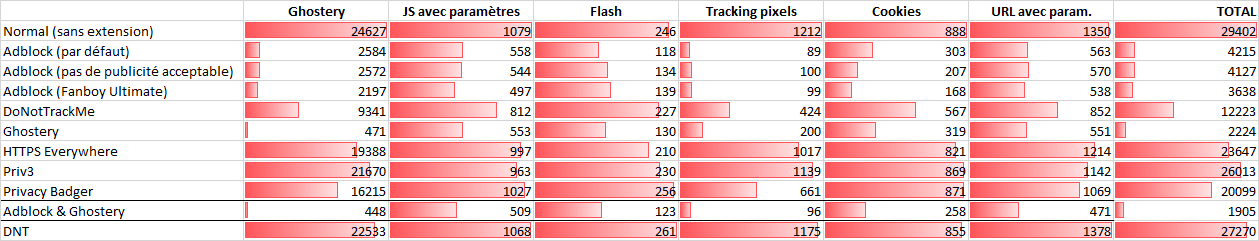
\includegraphics[scale=.54]{resultats/ANALYSES/Images/Comparaisons-Ghostery.png}
	\caption{\label{exp-DNT-ghostery}Comparaison des différents expériences (avec la base Ghostery).}
\end{figure}

\begin{figure}[!h]
	\hspace{-2cm}
	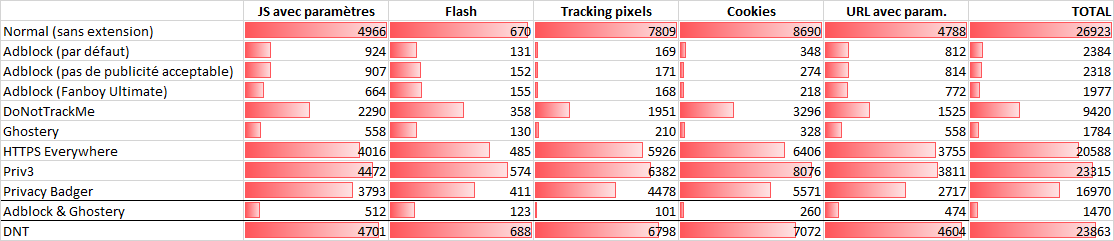
\includegraphics[scale=.6]{resultats/ANALYSES/Images/Comparaisons-NoG.png}
	\caption{\label{exp-DNT-ghostery}Comparaison des différents expériences (sans la base Ghostery).}
\end{figure}

Seule l'analyse utilisant la base de données Ghostery a été utilisée pour le calcul des résultats pour la raison évoquée dans la \autoref{extensions_navigateurs}. Cependant, ces deux tableaux permettent de constater que les deux types d'analyses fournissent proportionnellement les mêmes résultats sur les différentes expériences.
\newline

Ils permettent également de voir en un seul coup d'\oe{}il quelles sont les expériences qui donnent les meilleurs résultats.

La combinaison des extensions Adblock (avec la liste Fanboy Ultimate) et Ghostery offre la meilleure protection.

Si l'utilisateur ne désire installer qu'une seule extension, son choix devrait se porter sur Ghostery.
En effet, c'est l'extension qui obtient les meilleurs résultats même dans le type d'analyse qui n'utilise pas leur base de données. Elle est suivie par Adblock (équipée de la liste Fanboy Ultimate).

